\documentclass[12pt,a4paper]{article}

\usepackage[margin=2.2cm]{geometry}
\usepackage{fontspec}
\setmainfont{Times New Roman}
\usepackage{amsmath,amssymb,bm}
\usepackage{booktabs}
\usepackage{float}
\usepackage{graphicx}
\usepackage{caption}
\usepackage{setspace}
\captionsetup{font=small,labelfont=bf,skip=4pt}
\graphicspath{{figures/}}
\usepackage{hyperref}
\setstretch{1.08}
\raggedbottom

\hypersetup{colorlinks=true,linkcolor=black,urlcolor=blue,pdftitle={}}

\begin{document}

Problem~4.38 equips a dc-motor speed loop with the static feedforward gain \(K_{ff}=G_{\mathrm{nom}}^{-1}(0)\) and the proportional law \(k_p=3\).
On the nominal plant that choice makes the unit-step tracking gain equal to one and the dc gain from an output disturbance equal to zero.
The extension keeps those two designs fixed and asks what survives when the motor gain is wrong, when the disturbance is a step that the plant cannot cancel instantly, when the disturbance measurement is noisy, and when the same hardware is asked to track a reference and reject a later disturbance under a \(+15\%\) gain error.
The script is \texttt{hw05\_p3\_extension.m}. Every number below is taken from \texttt{simulation\_results.txt}.

%==============================================================================
\section{Closed-loop relations}

The nominal speed plant is
\begin{equation}
  G_{\mathrm{nom}}(s)=\frac{b}{s^2+as+c}
  =\frac{59.292}{s^2+6.978s+15.123},
  \label{eq:Gnom}
\end{equation}
with dc gain \(G_{\mathrm{nom}}(0)=b/c=3.920651\) and
\begin{equation}
  K_{ff}=\frac{c}{b}=0.25505970.
  \label{eq:Kff}
\end{equation}
A gain error is represented by \(G_{\mathrm{act}}(s)=(1+\delta)G_{\mathrm{nom}}(s)\): the poles of the motor stay put and only the numerator changes.
The measured signals available to the controller are the reference \(r\), the speed \(y\), and, when feedforward is used, the output disturbance \(w\). The plant equation is
\begin{equation}
  Y(s)=W(s)+G_{\mathrm{act}}(s)\,U(s).
  \label{eq:plant}
\end{equation}
The control law used throughout the extension is
\begin{equation}
  U(s)=D_c(s)\bigl(R(s)-Y(s)\bigr)+K_{ff,r}R(s)-K_{ff,w}W(s).
  \label{eq:law}
\end{equation}
Pure feedback sets both feedforward coefficients to zero.
Static feedforward sets both of them equal to \(K_{ff}\).
Two choices of \(D_c\) appear later: \(D_c=k_p\) and \(D_c=k_p+k_i/s\).

Eliminating \(U\) gives the two closed-loop maps
\begin{align}
  \frac{Y}{R}
  &=\frac{G_{\mathrm{act}}(D_c+K_{ff,r})}{1+D_c G_{\mathrm{act}}},
  \label{eq:YR}\\
  \frac{Y}{W}
  &=\frac{1-K_{ff,w}G_{\mathrm{act}}}{1+D_c G_{\mathrm{act}}}.
  \label{eq:YW}
\end{align}
The characteristic polynomial is \(1+D_c G_{\mathrm{act}}\). Neither \(K_{ff,r}\) nor \(K_{ff,w}\) enters it, so feedforward moves zeros and forced-response coefficients, not poles.

For \(D_c=k_p\) and \(K_{ff,r}=K_{ff,w}=K_{ff}\), the final-value theorem on a unit step produces the same dc number in both channels. With \(G_{\mathrm{act}}(0)=(1+\delta)G_{\mathrm{nom}}(0)\) and \(K_{ff}G_{\mathrm{nom}}(0)=1\),
\begin{equation}
  e_{ss}
  =1-T(0)
  =T_w(0)
  =\frac{-\delta}{1+k_p(1+\delta)G_{\mathrm{nom}}(0)}.
  \label{eq:ess}
\end{equation}
A positive \(\delta\) means the motor is stronger than the model used to build \(K_{ff}\). The fixed feedforward command is then too large, the speed settles above the reference, and \(e_{ss}\) is negative.
At \(\delta=0\), \eqref{eq:ess} is zero in both channels.
Without feedforward the same calculation leaves
\begin{equation}
  e_{ss}=T_w(0)=\frac{1}{1+k_p G_{\mathrm{act}}(0)},
  \label{eq:ess-p}
\end{equation}
which equals \(0.078358\) on the nominal motor.

The identity is stronger than a dc statement. For this proportional law,
\begin{equation}
  \left.\frac{E(s)}{R(s)}\right|_{W=0}
  =\left.\frac{Y(s)}{W(s)}\right|_{R=0}
  =\frac{1-K_{ff}G_{\mathrm{act}}(s)}{1+k_p G_{\mathrm{act}}(s)},
  \label{eq:identity}
\end{equation}
and the same equality holds with \(K_{ff}=0\).
A unit-step tracking error and a unit-step disturbance response are therefore the same waveform.
Integrated absolute error, settling time, and the relation between the tracking peak and the disturbance undershoot have to agree for that reason, not because two experiments happened to land on the same digits.

On the nominal motor the proportional loop is second order,
\begin{equation}
  s^2+as+\bigl(c+k_p b\bigr)
  =s^2+6.978s+192.999,
  \label{eq:charP}
\end{equation}
with \(\omega_n=13.8924~\mathrm{rad/s}\) and \(\zeta=0.2511\).
The closed-loop poles are \(-3.4890\pm 13.4472j\).
The real part \(-a/2=-3.489\) does not depend on \(b\) or on \(\delta\).
Changing the motor gain changes \(\omega_n\) and \(\zeta\), but it does not change the exponential envelope \(e^{-3.489t}\).
The two nominal transfer functions collapse to
\begin{align}
  T(s)&=\frac{192.999}{s^2+6.978s+192.999},
  \label{eq:Tnom}\\
  T_w(s)&=\frac{s(s+6.978)}{s^2+6.978s+192.999}.
  \label{eq:Twnom}
\end{align}
The pure-P tracking map is the same denominator with numerator \(k_p b=177.876\).
Feedforward therefore multiplies the entire nominal tracking response by
\begin{equation}
  \frac{k_p+K_{ff}}{k_p}=1.085020.
  \label{eq:scale}
\end{equation}
The simulated check of this identity, \(\max|y_{ff}(t)-1.085020\,y_P(t)|\), is \(1.332\times 10^{-14}\).

%==============================================================================
\section{Experimental method}

The motor is integrated in controllable canonical form,
\[
  \dot x=\begin{bmatrix}0&1\\-c&-a\end{bmatrix}x
  +\begin{bmatrix}0\\(1+\delta)b\end{bmatrix}u,
  \qquad
  y=x_1+w.
\]
A proportional integrator, when used, adds the state \(\dot\xi=r-y\).
Inputs are held constant between samples and the state transition is the exact matrix exponential of that hold, with \(dt=10^{-3}~\mathrm{s}\) and a horizon of \(5~\mathrm{s}\).
On a piecewise-constant input the samples match the continuous-time response.
The largest discrepancy between \eqref{eq:ess} and the simulated endpoint, over the seven gain errors of Section~\ref{sec:mismatch}, is \(2.6\times 10^{-8}\).

Settling and recovery use an absolute band of \(0.02\), which is \(2\%\) of a unit step.
The settling time is the first instant after which the signal remains inside that band about its theoretical steady value.
Overshoot is \((y_{\mathrm{peak}}-y_{ss})/|y_{ss}|\times 100\%\), reported as zero when the peak does not exceed the steady value.
Recovery time in the two-phase test is the same band about \(y=1\), measured from the disturbance instant \(t=2.5~\mathrm{s}\).

The integral gain is chosen with \(k_p\) held at 3, so the proportional and PI architectures differ only by the integrator and the feedforward terms.
On the nominal motor the PI characteristic polynomial is
\begin{equation}
  s^3+as^2+(c+bk_p)s+bk_i,
  \label{eq:charPI}
\end{equation}
and the Routh margin is \(a(c+bk_p)-bk_i\).
Table~\ref{tab:ki} is that calculation.
\(k_i=15\) is stable, but its complex pair has \(\zeta=0.078\), far below the proportional loop's \(\zeta=0.251\).
The working value is \(k_i=4\), where \(\zeta=0.209\) and the real pole is \(-1.277\).
That real pole is fast enough for the tracking transient to be essentially over before the disturbance at \(2.5~\mathrm{s}\), which is the comparison the two-phase test is built to make.

\begin{table}[H]
  \centering
  \caption{Nominal PI candidates with \(k_p=3\). The margin is \(a(c+bk_p)-bk_i\). The run uses \(k_i=4\).}
  \label{tab:ki}
  \begin{tabular}{cccc}
    \toprule
    \(k_i\) & Routh margin & \(\zeta\) of the complex pair & Real pole \\
    \midrule
    \(2\)  & \(1228.16\) & \(0.231\) & \(-0.627\) \\
    \(4\)  & \(1109.58\) & \(0.209\) & \(-1.277\) \\
    \(15\) & \(457.37\)  & \(0.078\) & \(-4.867\) \\
    \bottomrule
  \end{tabular}
\end{table}

Disturbance-sensor noise is discrete and white at the simulation step: each sample of \(n\) is independent, zero mean, and of standard deviation \(\sigma=0.05\), with the generator seeded at \(20261022\).
It is not a continuous white noise of unit spectral density.
The filter compared against the raw measurement is the causal low-pass \(H(s)=20/(s+20)\), a time constant of \(50~\mathrm{ms}\).
The controller sees \(\hat w\); the plant is still driven by the true \(w\). Feedback continues to use the true \(y\), so this noise enters only through the feedforward term.

%==============================================================================
\section{Perfect-model baseline}

Figure~\ref{fig:base} and Table~\ref{tab:base} compare pure P with P plus static feedforward on \(G_{\mathrm{nom}}\).
Tracking uses \(r=1(t)\) and \(w=0\). Disturbance rejection uses \(r=0\) and \(w=1(t)\).

\begin{table}[H]
  \centering
  \caption{Nominal unit-step tests. Overshoot is relative to each response's own steady value. \(T_s\) uses the band \(0.02\) about that value. The two blocks are the same waveforms, by \eqref{eq:identity}.}
  \label{tab:base}
  \small
  \setlength{\tabcolsep}{5pt}
  \begin{tabular}{lcc}
    \toprule
    Quantity & Pure P & P + feedforward \\
    \midrule
    Tracking \(e_{ss}\) (theory and simulation) & \(0.078358\) & \(0\) \\
    \(y_{\mathrm{peak}}\) and its time & \(1.3295\) at \(0.234~\mathrm{s}\) & \(1.4426\) at \(0.234~\mathrm{s}\) \\
    Overshoot about \(y_{ss}\) & \(44.26\%\) & \(44.26\%\) \\
    Amount by which the peak exceeds \(1\) & \(33.0\%\) & \(44.3\%\) \\
    \(T_s\) about \(y_{ss}\) & \(1.011~\mathrm{s}\) & \(1.016~\mathrm{s}\) \\
    Time to enter and stay in \(|y-1|<0.02\) & never & \(1.016~\mathrm{s}\) \\
    \(\int_0^5 |1-y|\,dt\) & \(0.5102\) & \(0.1970\) \\
    \(u(\infty)\) & \(0.2351\) & \(0.2551\) \\
    \midrule
    Disturbance \(y(0^+)\) & \(1\) & \(1\) \\
    Disturbance \(y_{ss}\) & \(0.078358\) & \(0\) \\
    \(y_{\min}\) and its time & \(-0.3295\) at \(0.234~\mathrm{s}\) & \(-0.4426\) at \(0.234~\mathrm{s}\) \\
    \(\int_0^5 |y|\,dt\) & \(0.5102\) & \(0.1970\) \\
    \(u(0^+)\) and \(u(\infty)\) & \(-3\), \(-0.2351\) & \(-3.2551\), \(-0.2551\) \\
    \bottomrule
  \end{tabular}
\end{table}

\begin{figure}[H]
  \centering
  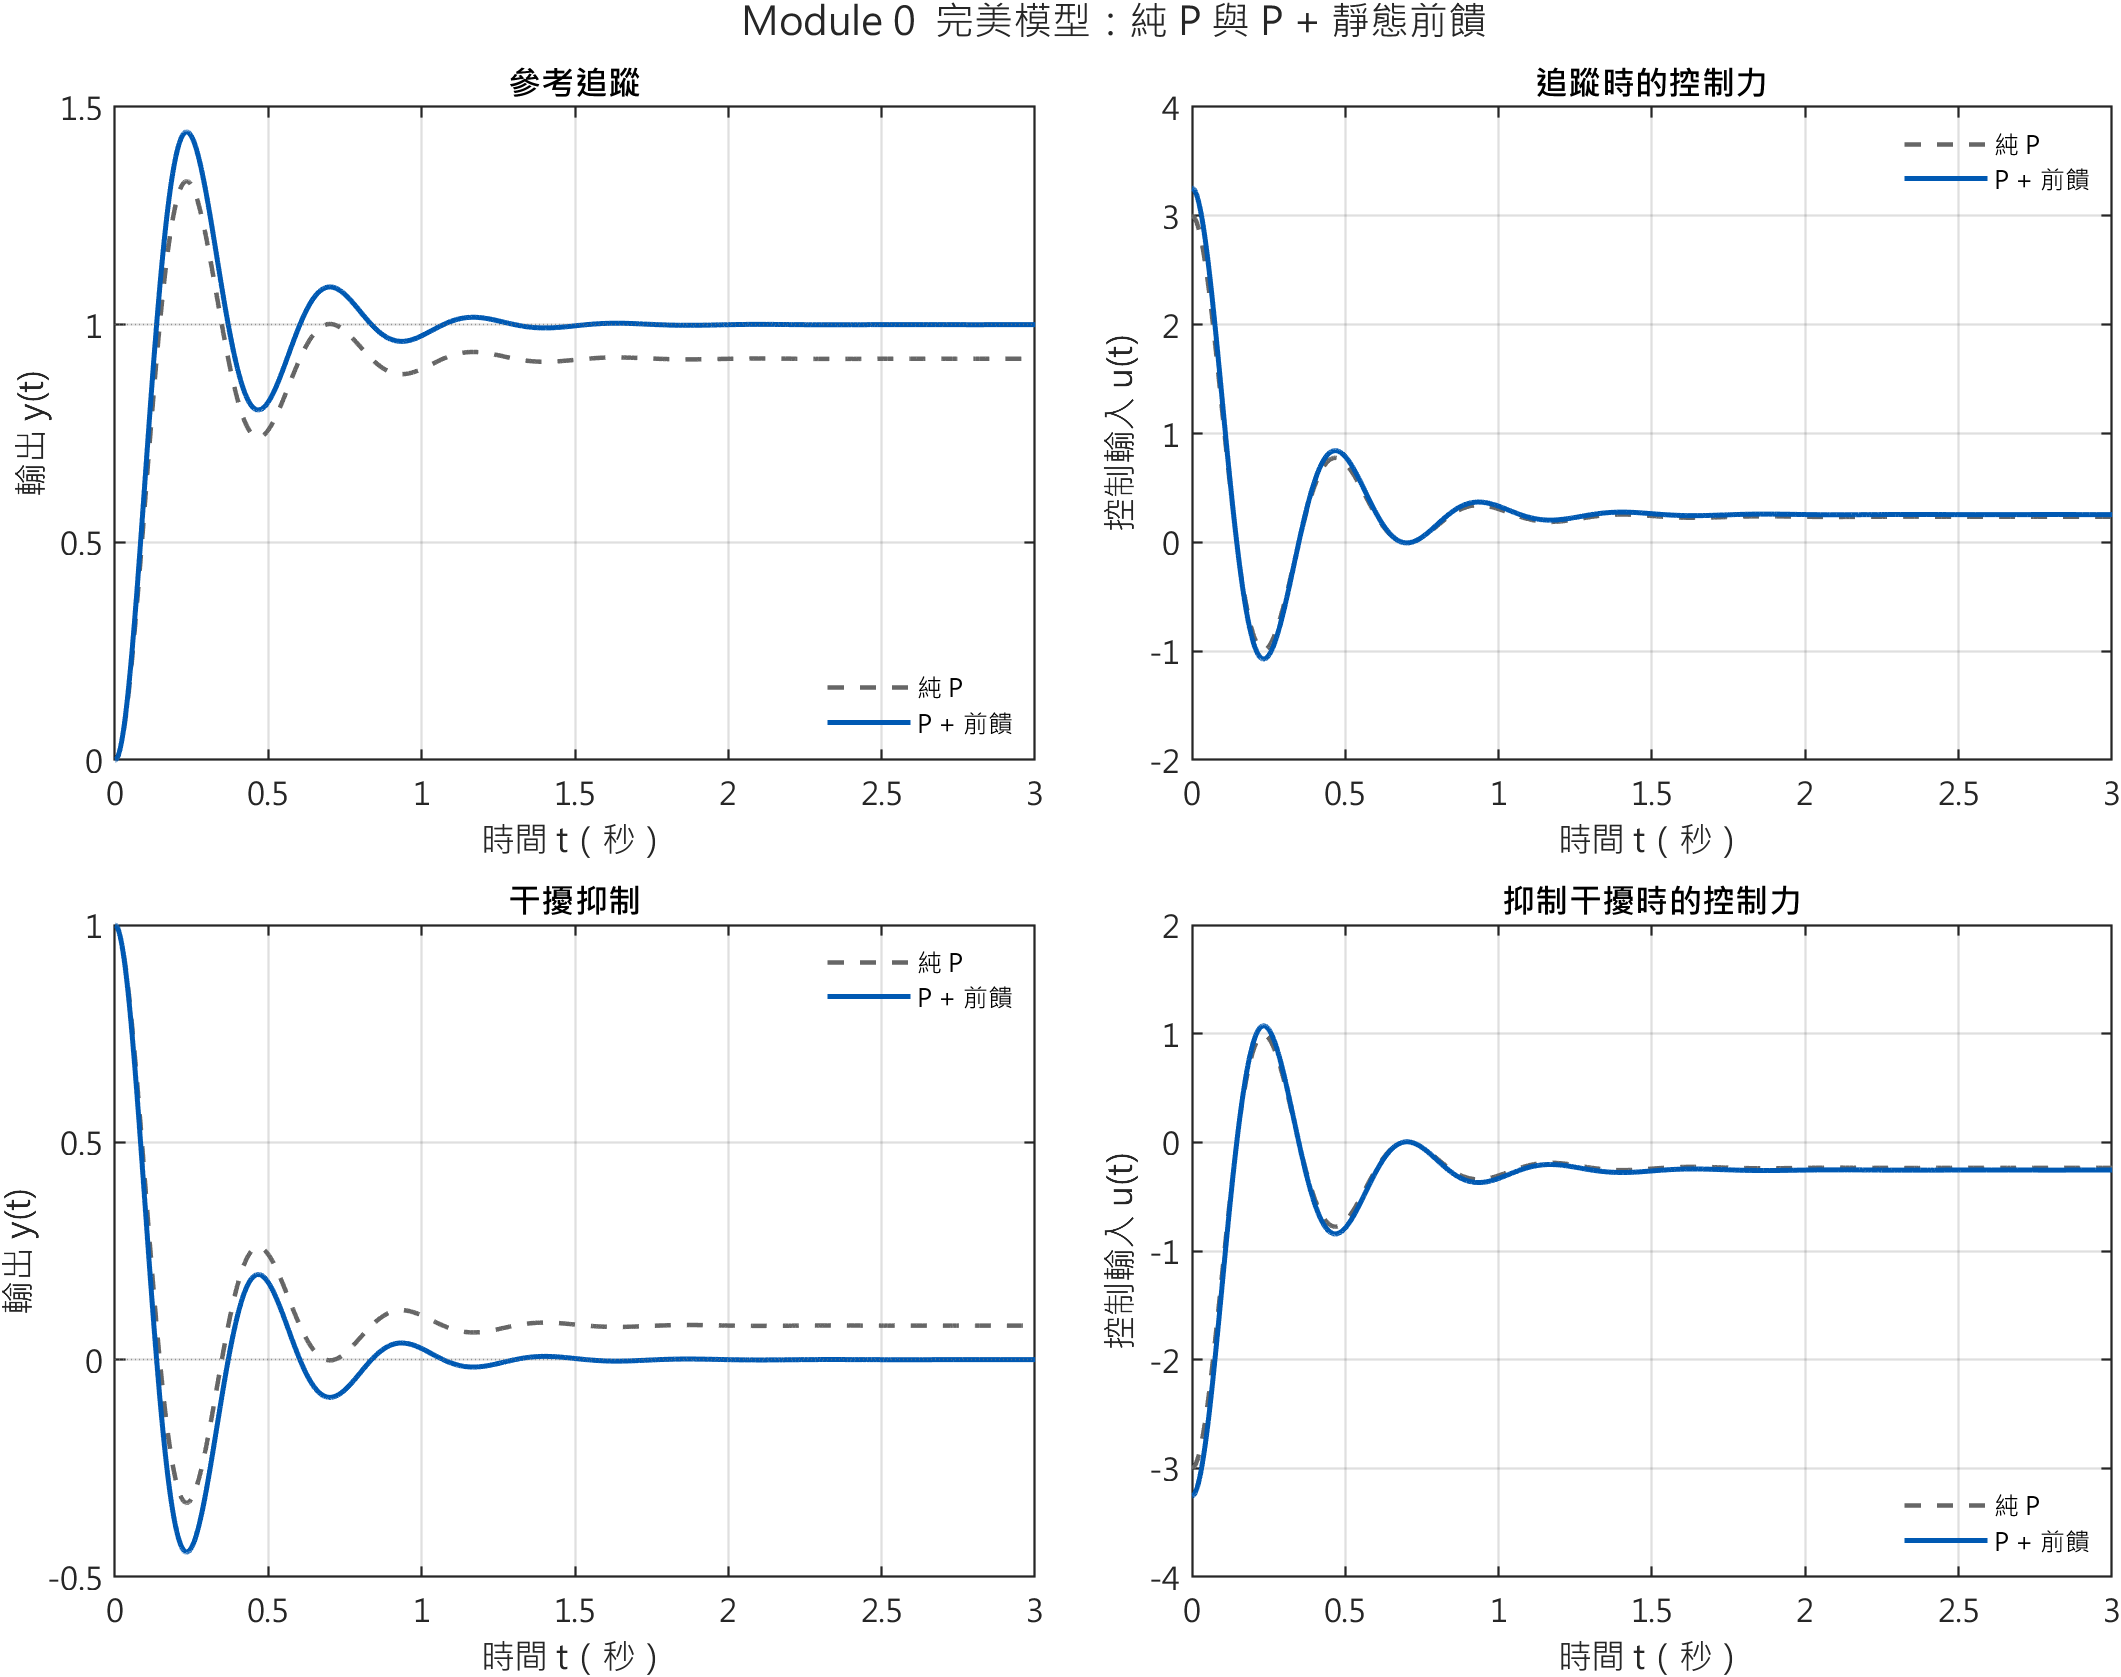
\includegraphics[width=\textwidth]{fig0_baseline.png}
  \caption{Nominal plant. Dashed: \(k_p=3\) alone. Solid: the same \(k_p\) plus \(K_{ff}\).
  The tracking pair differs by the constant factor \eqref{eq:scale}. The disturbance pair starts at the same value \(1\) and separates at steady state.}
  \label{fig:base}
\end{figure}

Feedforward removes the \(7.84\%\) steady tracking error and cuts the integrated absolute error from \(0.510\) to \(0.197\), a reduction of \(61\%\).
It does this without moving the peak time. Both tracking peaks occur at \(0.234~\mathrm{s}\), and both overshoots about their own steady values are \(44.26\%\), as required by \eqref{eq:scale}.
What does change is the absolute excursion past the reference: the pure-P peak is \(1.330\), which is \(0.330\) above \(1\), while the feedforward peak is \(1.443\).
Pure P also never enters the band \(|y-1|<0.02\), because its steady error \(0.078\) is already outside that band. Feedforward enters the band at \(1.016~\mathrm{s}\) and stays there.
The steady control effort moves from \(k_p e_{ss}=0.235\) to \(K_{ff}=0.255\). Once the error is zero, the loop holds exactly the model inverse of the speed command.

The disturbance column is the tracking-error column read through \eqref{eq:identity}.
The integrated areas match to all printed digits, the settling times match, and
\[
  y_{\mathrm{dist,min}}=1-y_{\mathrm{track,peak}}.
\]
For feedforward, \(1-1.442581=-0.442581\).
The undershoot is the tracking overshoot, seen from the other side of the same loop.
Feedforward deepens it, from \(-0.330\) to \(-0.443\), because the same scale factor that lifts the tracking peak pushes the disturbance waveform further negative. It is also what brings \(y(\infty)\) from \(0.078\) to \(0\), and the disturbance IAE falls by the same \(61\%\).

%==============================================================================
\section{Frozen feedforward under gain error}
\label{sec:mismatch}

\(K_{ff}\) is left at the nominal inverse while \(\delta\) runs through \(\{\pm 20,\pm 10,\pm 5,0\}\%\).
Figure~\ref{fig:mis} shows the family. Table~\ref{tab:mis} gives the tracking metrics; the disturbance steady values are the same numbers by \eqref{eq:ess}, and the simulated disturbance minima satisfy \(y_{\min}=1-y_{\mathrm{peak}}\) at every listed \(\delta\).

\begin{table}[H]
  \centering
  \caption{P + nominal \(K_{ff}\) on \(G_{\mathrm{act}}=(1+\delta)G_{\mathrm{nom}}\). Theory is \eqref{eq:ess}. Overshoot is about the theoretical \(y_{ss}=1-e_{ss}\). \(T_s\) is the \(0.02\) band about that value.}
  \label{tab:mis}
  \small
  \setlength{\tabcolsep}{5pt}
  \begin{tabular}{rrrrrr}
    \toprule
    \(\delta\) & \(e_{ss}\) theory & \(e_{ss}\) simulated & \(y_{\mathrm{peak}}\) & Overshoot & \(T_s\) (s) \\
    \midrule
    \(-20\%\) & \(+0.019213\) & \(+0.019213\) & \(1.3758\) & \(40.27\%\) & \(1.102\) \\
    \(-10\%\) & \(+0.008631\) & \(+0.008631\) & \(1.4115\) & \(42.38\%\) & \(1.058\) \\
    \(-5\%\)  & \(+0.004107\) & \(+0.004107\) & \(1.4276\) & \(43.35\%\) & \(1.037\) \\
    \(0\)     & \(0\)         & \(0\)         & \(1.4426\) & \(44.26\%\) & \(1.016\) \\
    \(+5\%\)  & \(-0.003745\) & \(-0.003745\) & \(1.4567\) & \(45.12\%\) & \(0.996\) \\
    \(+10\%\) & \(-0.007175\) & \(-0.007175\) & \(1.4699\) & \(45.94\%\) & \(1.132\) \\
    \(+20\%\) & \(-0.013232\) & \(-0.013232\) & \(1.4942\) & \(47.47\%\) & \(1.111\) \\
    \bottomrule
  \end{tabular}
\end{table}

\begin{figure}[H]
  \centering
  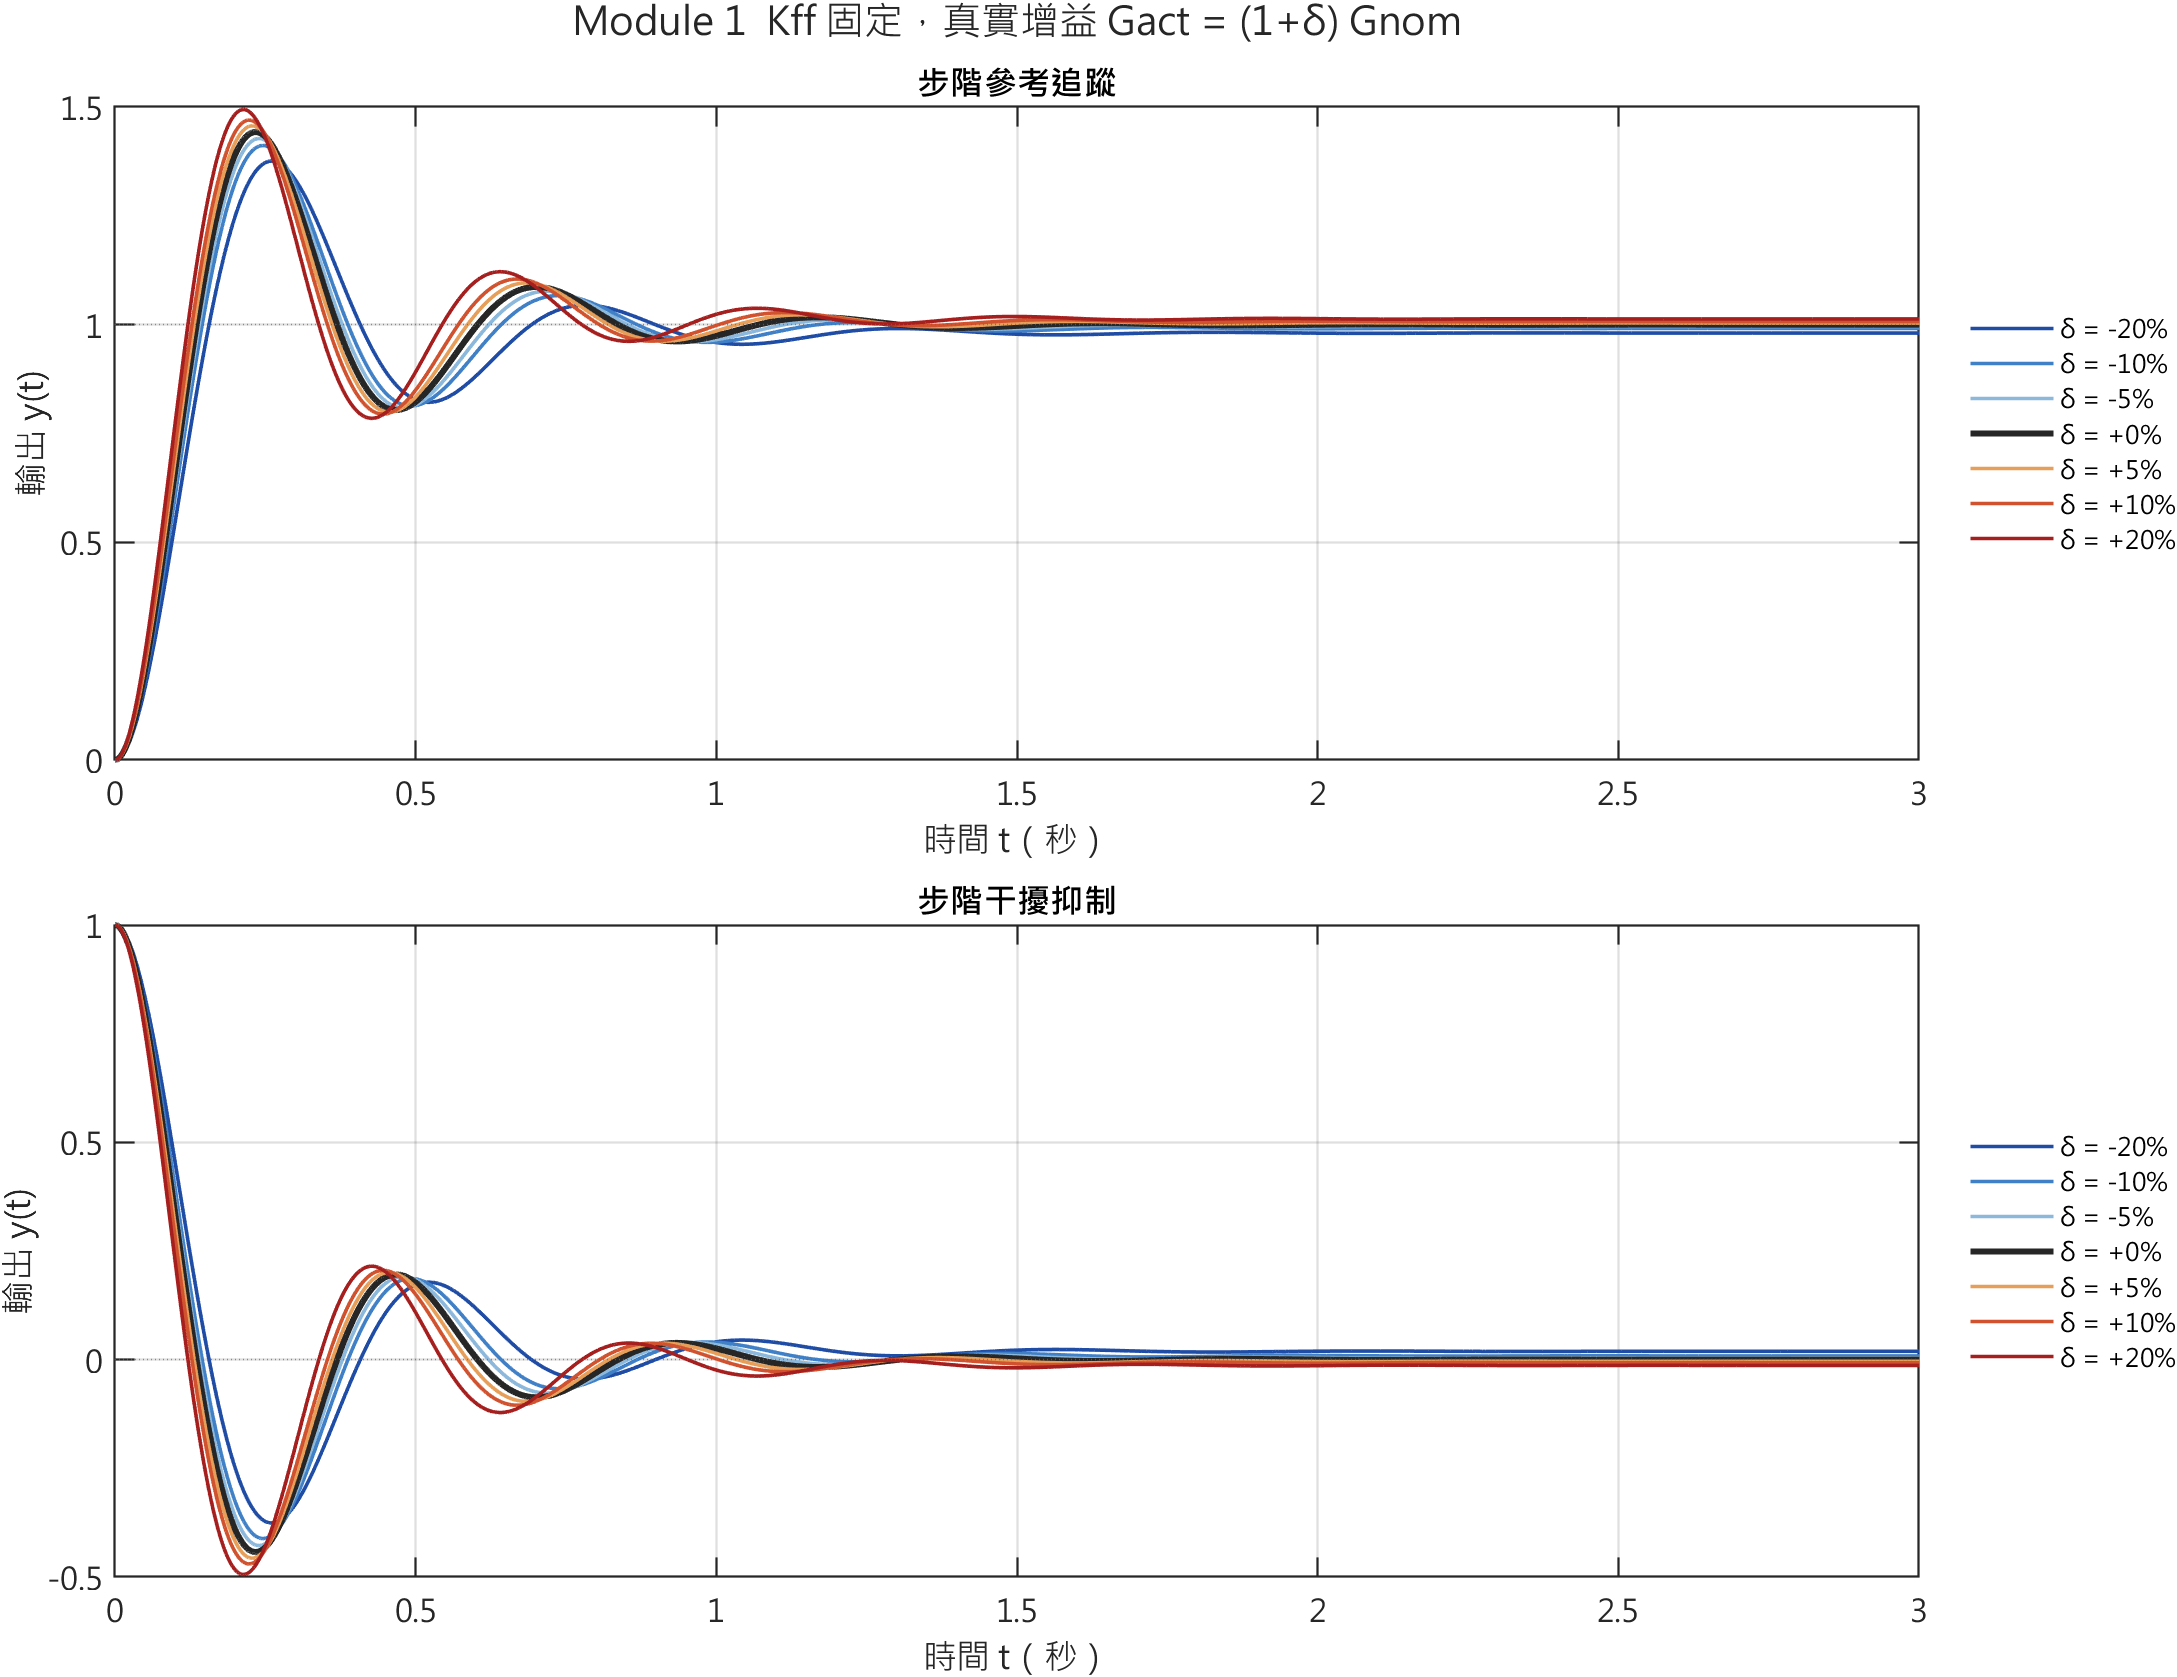
\includegraphics[width=\textwidth]{fig1_gain_mismatch.png}
  \caption{Frozen \(K_{ff}\), motor gain \((1+\delta)\) times nominal.
  Upper: reference step. Lower: output-disturbance step.
  Blue is a weak motor, red is a strong motor, and the black curve is \(\delta=0\).
  The transients stay together; the steady levels split by \eqref{eq:ess}.}
  \label{fig:mis}
\end{figure}

A \(20\%\) model error does not become a \(20\%\) speed error.
The proportional loop gain at dc is \(k_p G_{\mathrm{nom}}(0)=11.762\), so \(1+k_p G_{\mathrm{nom}}(0)=12.762\).
For small \(\delta\), \eqref{eq:ess} is approximately \(-\delta/12.762\): feedback attenuates the feedforward's dc mistake by the sensitivity \(1/(1+k_p G(0))\).
The \(\pm 20\%\) residuals are \(+1.92\%\) and \(-1.32\%\). The two magnitudes differ because the denominator of \eqref{eq:ess} itself depends on \(\delta\); a stronger motor gives a larger loop gain and a smaller residual.
The sign follows the inverse used in \(K_{ff}\). On a strong motor the nominal inverse commands too much input, \(y_{ss}>1\), and the error is negative. On a weak motor the command is too small and the speed settles low.

The curves in Fig.~\ref{fig:mis} separate much less at steady state than they do at the first peak.
The peak rises from \(1.376\) at \(\delta=-20\%\) to \(1.494\) at \(\delta=+20\%\), and the overshoot about \(y_{ss}\) rises from \(40.3\%\) to \(47.5\%\).
That trend is the damping ratio. The closed-loop polynomial is \(s^2+as+(c+k_p(1+\delta)b)\), so
\[
  \omega_n=\sqrt{c+k_p(1+\delta)b},\qquad
  \zeta=\frac{a}{2\omega_n}.
\]
At the two ends of the sweep, \((\omega_n,\zeta)\) moves from \((12.55,\,0.278)\) to \((15.12,\,0.231)\).
Higher gain raises the natural frequency and lowers the damping ratio, which is the larger overshoot.
The product \(\zeta\omega_n=a/2=3.489\) is the same at every \(\delta\).
The envelope decays at one common rate, which is why \(T_s\) stays inside \(0.996\)--\(1.132~\mathrm{s}\) across a \(\pm 20\%\) gain change.
The small non-monotonic wiggle in \(T_s\) is the \(2\%\) band meeting a slightly different oscillatory phase, not a change in the decay rate.
The same real part is visible again in Section~\ref{sec:arch}: under a \(+15\%\) error the proportional poles are still \(-3.4890\pm j\,14.4051\).

The practical reading is that static feedforward on this loop is accurate at dc only when the gain is right, but the proportional loop makes the dc penalty first-order small.
A \(\pm 20\%\) gain tolerance, if it is the dominant model error, leaves a steady speed error inside \(2\%\).
It does not buy a better damped transient. The overshoot moves by about seven percentage points over that same tolerance, and it moves in the direction of the gain error.

%==============================================================================
\section{Output-disturbance spike and measurement noise}
\label{sec:spike}

The disturbance in \eqref{eq:plant} is added to the speed, not to the motor input.
\(G_{\mathrm{act}}\) has relative degree \(2\), so a finite \(u\) cannot change \(y\) at the instant \(w\) jumps.
The initial-value theorem on \eqref{eq:Twnom} gives
\[
  y(0^+)=\lim_{s\to\infty}T_w(s)=1
\]
with or without feedforward. The simulation returns \(y(0)=1.000000\) in both cases.
The step \(w\) has zero slope after the jump, and the motor output and its derivative are still zero, so \(y'(0^+)=0\).
The first nonzero derivative is the motor acceleration,
\begin{equation}
  y''(0^+)=b\,u(0^+).
  \label{eq:ydd}
\end{equation}
With feedforward, \(u(0^+)=-(k_p+K_{ff})=-3.255060\) and \(y''(0^+)=-192.999\), which is \(-\omega_n^2\) for the nominal loop.
Without feedforward, \(u(0^+)=-k_p=-3\) and the initial curvature is only \(-k_p b=-177.876\).
The speed therefore leaves the spike horizontally and bends downward. Because \(\zeta=0.251\), it crosses the steady value and undershoots.
Figure~\ref{fig:spike} shows the bend, the undershoot, and the control effort that produces them.

\begin{figure}[H]
  \centering
  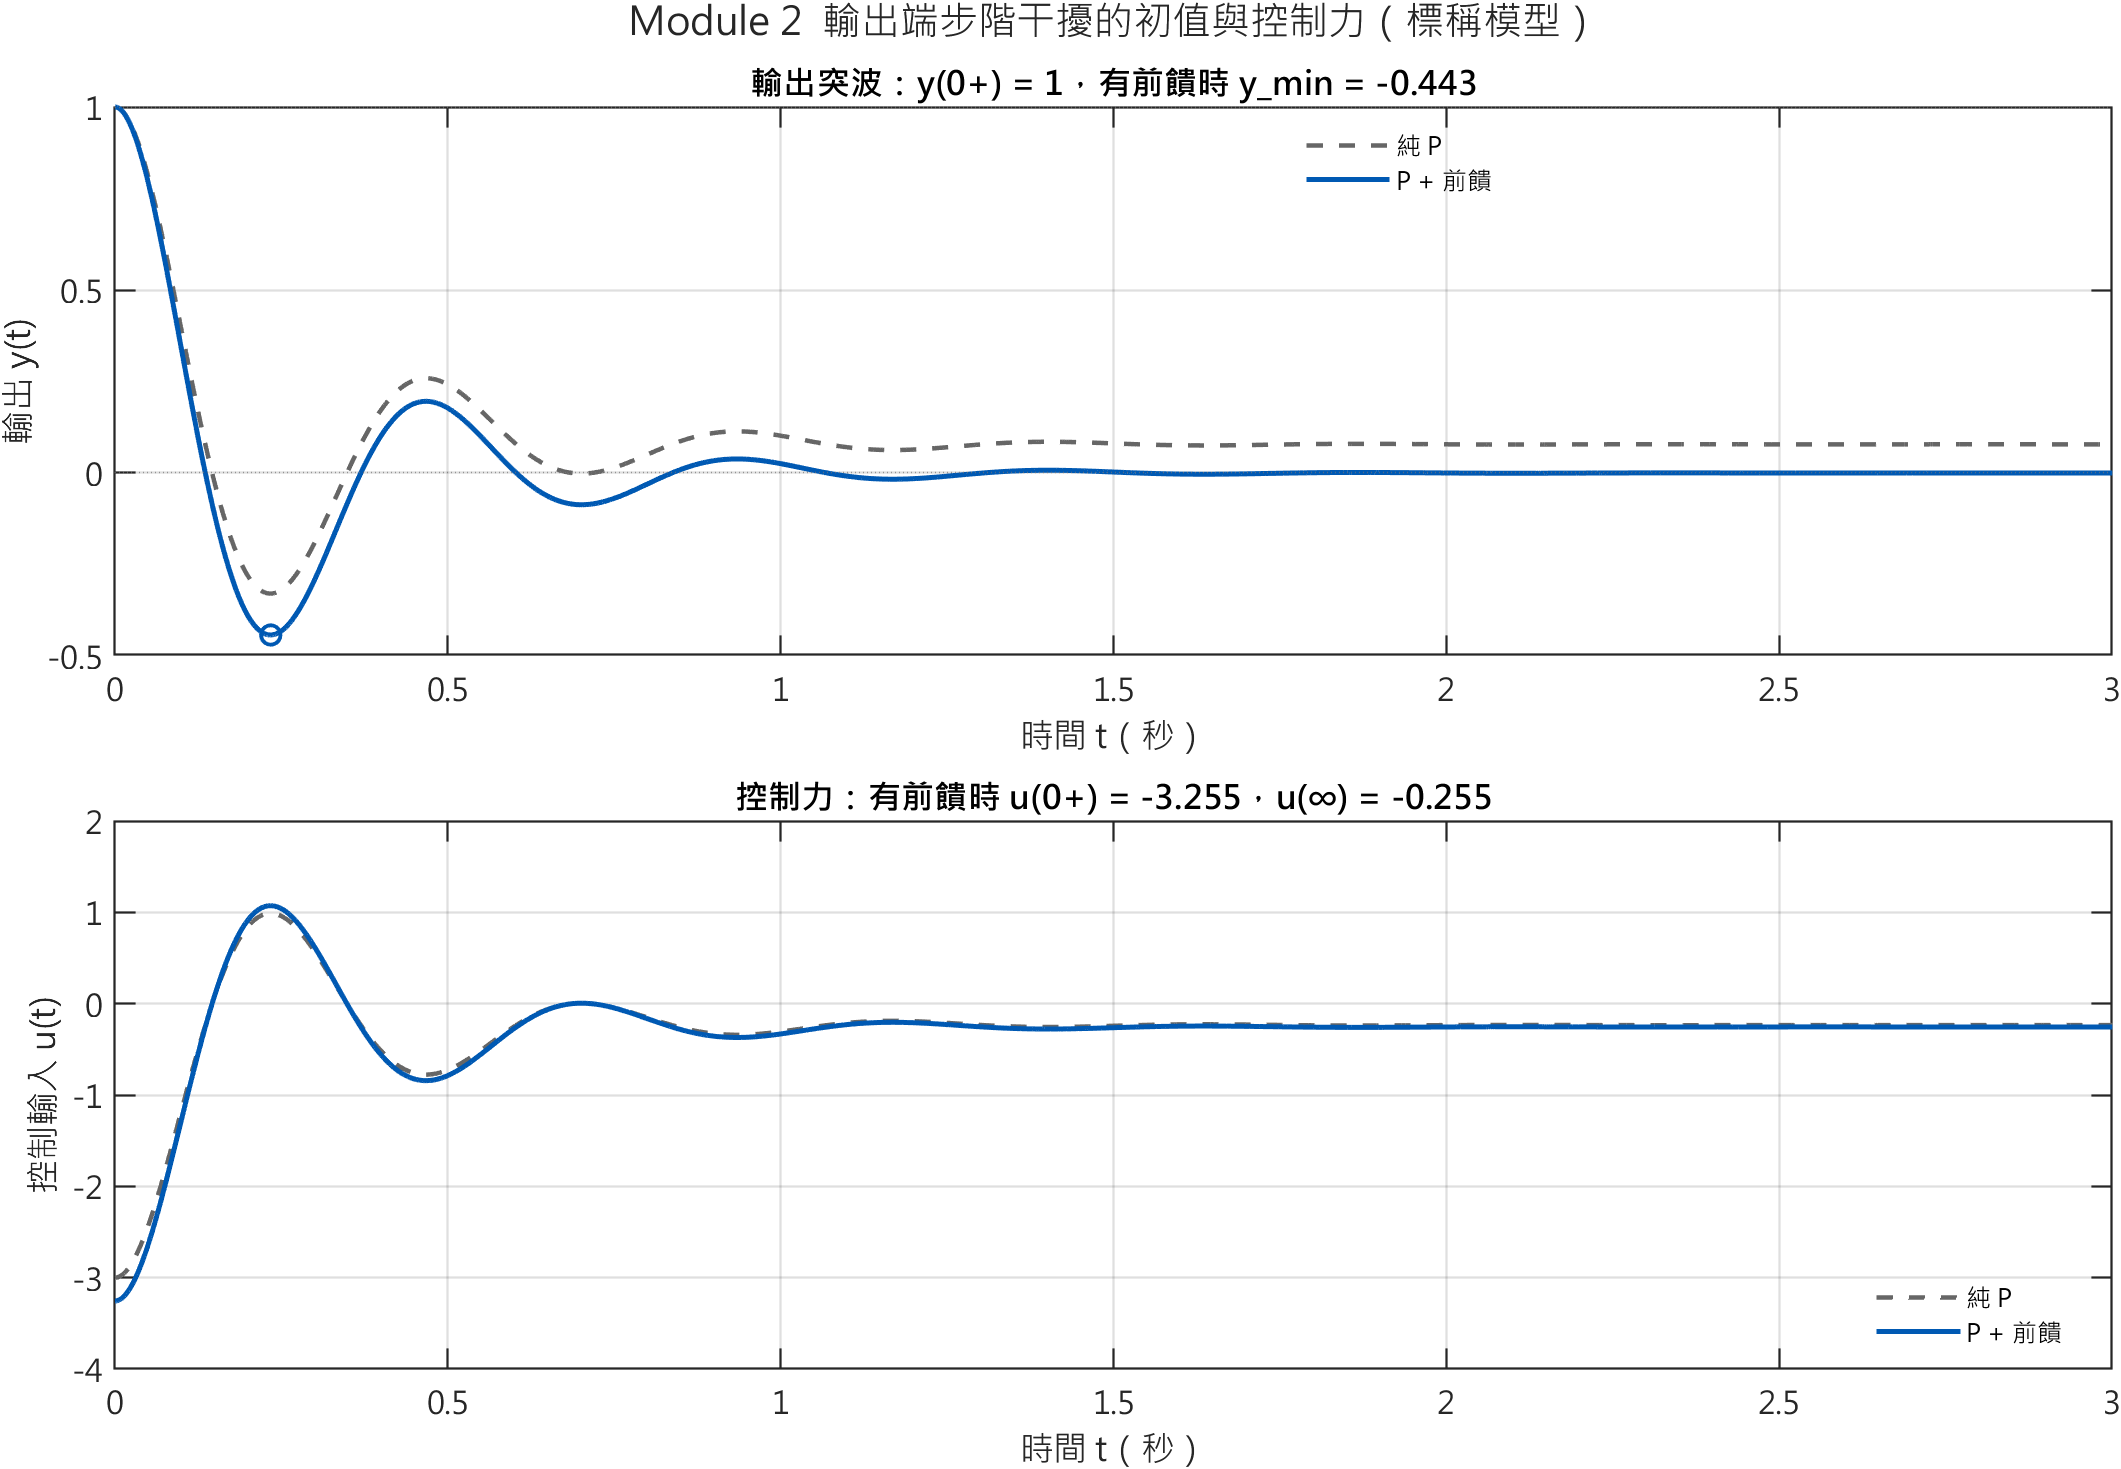
\includegraphics[width=\textwidth]{fig2_disturbance_spike.png}
  \caption{Nominal output-disturbance step.
  Both speeds start at \(1\). Feedforward is the curve that returns to \(0\) and reaches \(y_{\min}=-0.443\) at \(0.234~\mathrm{s}\).
  Its control effort starts at \(-3.255\) and settles at \(-K_{ff}=-0.255\).}
  \label{fig:spike}
\end{figure}

The numerator of \eqref{eq:Twnom} supplies the rest of the shape.
Perfect cancellation puts zeros at \(s=0\) and \(s=-6.978\).
The zero at the origin is the dc rejection. It does not cancel the complex poles, so the transient that carries \(y\) from \(1\) down to \(0\) is the same underdamped pair that produces the \(44\%\) tracking overshoot, arriving at the same time \(0.234~\mathrm{s}\).
After the transient, \(u(\infty)=-K_{ff}\) and the feedback effort is zero: the feedforward term alone holds the input that cancels a constant output disturbance on the nominal motor.
The pure-P loop has no such term, so it can hold \(y(\infty)=0.078\) only by a continuing feedback effort \(u(\infty)=-0.235\).

The spike is therefore not an artifact of feedforward. Feedforward changes the depth of the undershoot and the value at which the speed settles.
Any controller that sees \(y\) only through a strictly proper plant will show \(y(0^+)=1\) for this class of disturbance.
Cancelling the spike would require a feedthrough path around the motor, which this plant does not have.

The linear model also assumes the voltage command can take the value \(u(0^+)=-3.255\).
A dc-motor drive saturates. Rails of \(\pm 3~\mathrm{V}\) or \(\pm 5~\mathrm{V}\) are typical.
In the normalized units used here, every feedforward peak in this study lies between \(3.00\) and \(3.27\), so a \(\pm 5~\mathrm{V}\) limit still contains them and the linear maps remain valid.
A \(\pm 3~\mathrm{V}\) limit does not. The command stops at \(-3\), the extra \(-K_{ff}\) never reaches the armature, and the initial curvature in \eqref{eq:ydd} becomes \(-k_p b=-177.876\) rather than \(-192.999\).
Until \(u\) re-enters the rails, \eqref{eq:YW} ceases to describe the speed, and the dc cancellation that \(K_{ff}\) was computed to provide is only partly delivered.
Figure~\ref{fig:spike} is the unsaturated prediction. A drive limited to \(\pm 3~\mathrm{V}\) has to be resimulated with the saturation in the loop before the undershoot and the \(61\%\) drop in integrated absolute error are treated as hardware results.

Measurement noise is a separate question, because the feedforward path uses \(\hat w=w+n\).
From the high-frequency end of \eqref{eq:YW} and the matching expression for \(U\), a high-frequency component of \(n\) reaches the actuator with gain \(-K_{ff}\), not with gain \(-k_p\).
Since \(K_{ff}=0.255<1\), this sensor is attenuated on its way into \(u\).
At dc the same path is smaller still, by the factor \(1+k_p G_{\mathrm{nom}}(0)=12.762\).
Most of the energy of discrete white noise sampled at \(1~\mathrm{ms}\) sits near the Nyquist frequency, where the plant is already negligible, so the steady jitter of \(u\) should lie close to \(K_{ff}\sigma=0.01275\).

\begin{table}[H]
  \centering
  \caption{Nominal feedforward disturbance response with \(\sigma=0.05\) on \(\hat w\).
  Steady jitter is the rms of the signal about its own mean on \([3,5]~\mathrm{s}\).
  The full-horizon rms of \(u\) is dominated by the deterministic spike.}
  \label{tab:noise}
  \small
  \setlength{\tabcolsep}{4pt}
  \begin{tabular}{lrrrrr}
    \toprule
    Case & rms\((u)\) on \([0,5]\) & \(\max|u|\) & Steady rms of \(u\) & Steady rms of \(y\) & \(y_{\min}\) \\
    \midrule
    No noise        & \(0.4885\) & \(3.2551\) & \(1.8\times 10^{-5}\) & \(6\times 10^{-6}\) & \(-0.4426\) \\
    Noise, no filter & \(0.4887\) & \(3.2697\) & \(0.01292\) & \(5.05\times 10^{-4}\) & \(-0.4426\) \\
    Noise + low-pass & \(0.4769\) & \(3.0204\) & \(0.00149\) & \(4.41\times 10^{-4}\) & \(-0.4278\) \\
    \bottomrule
  \end{tabular}
\end{table}

\begin{figure}[H]
  \centering
  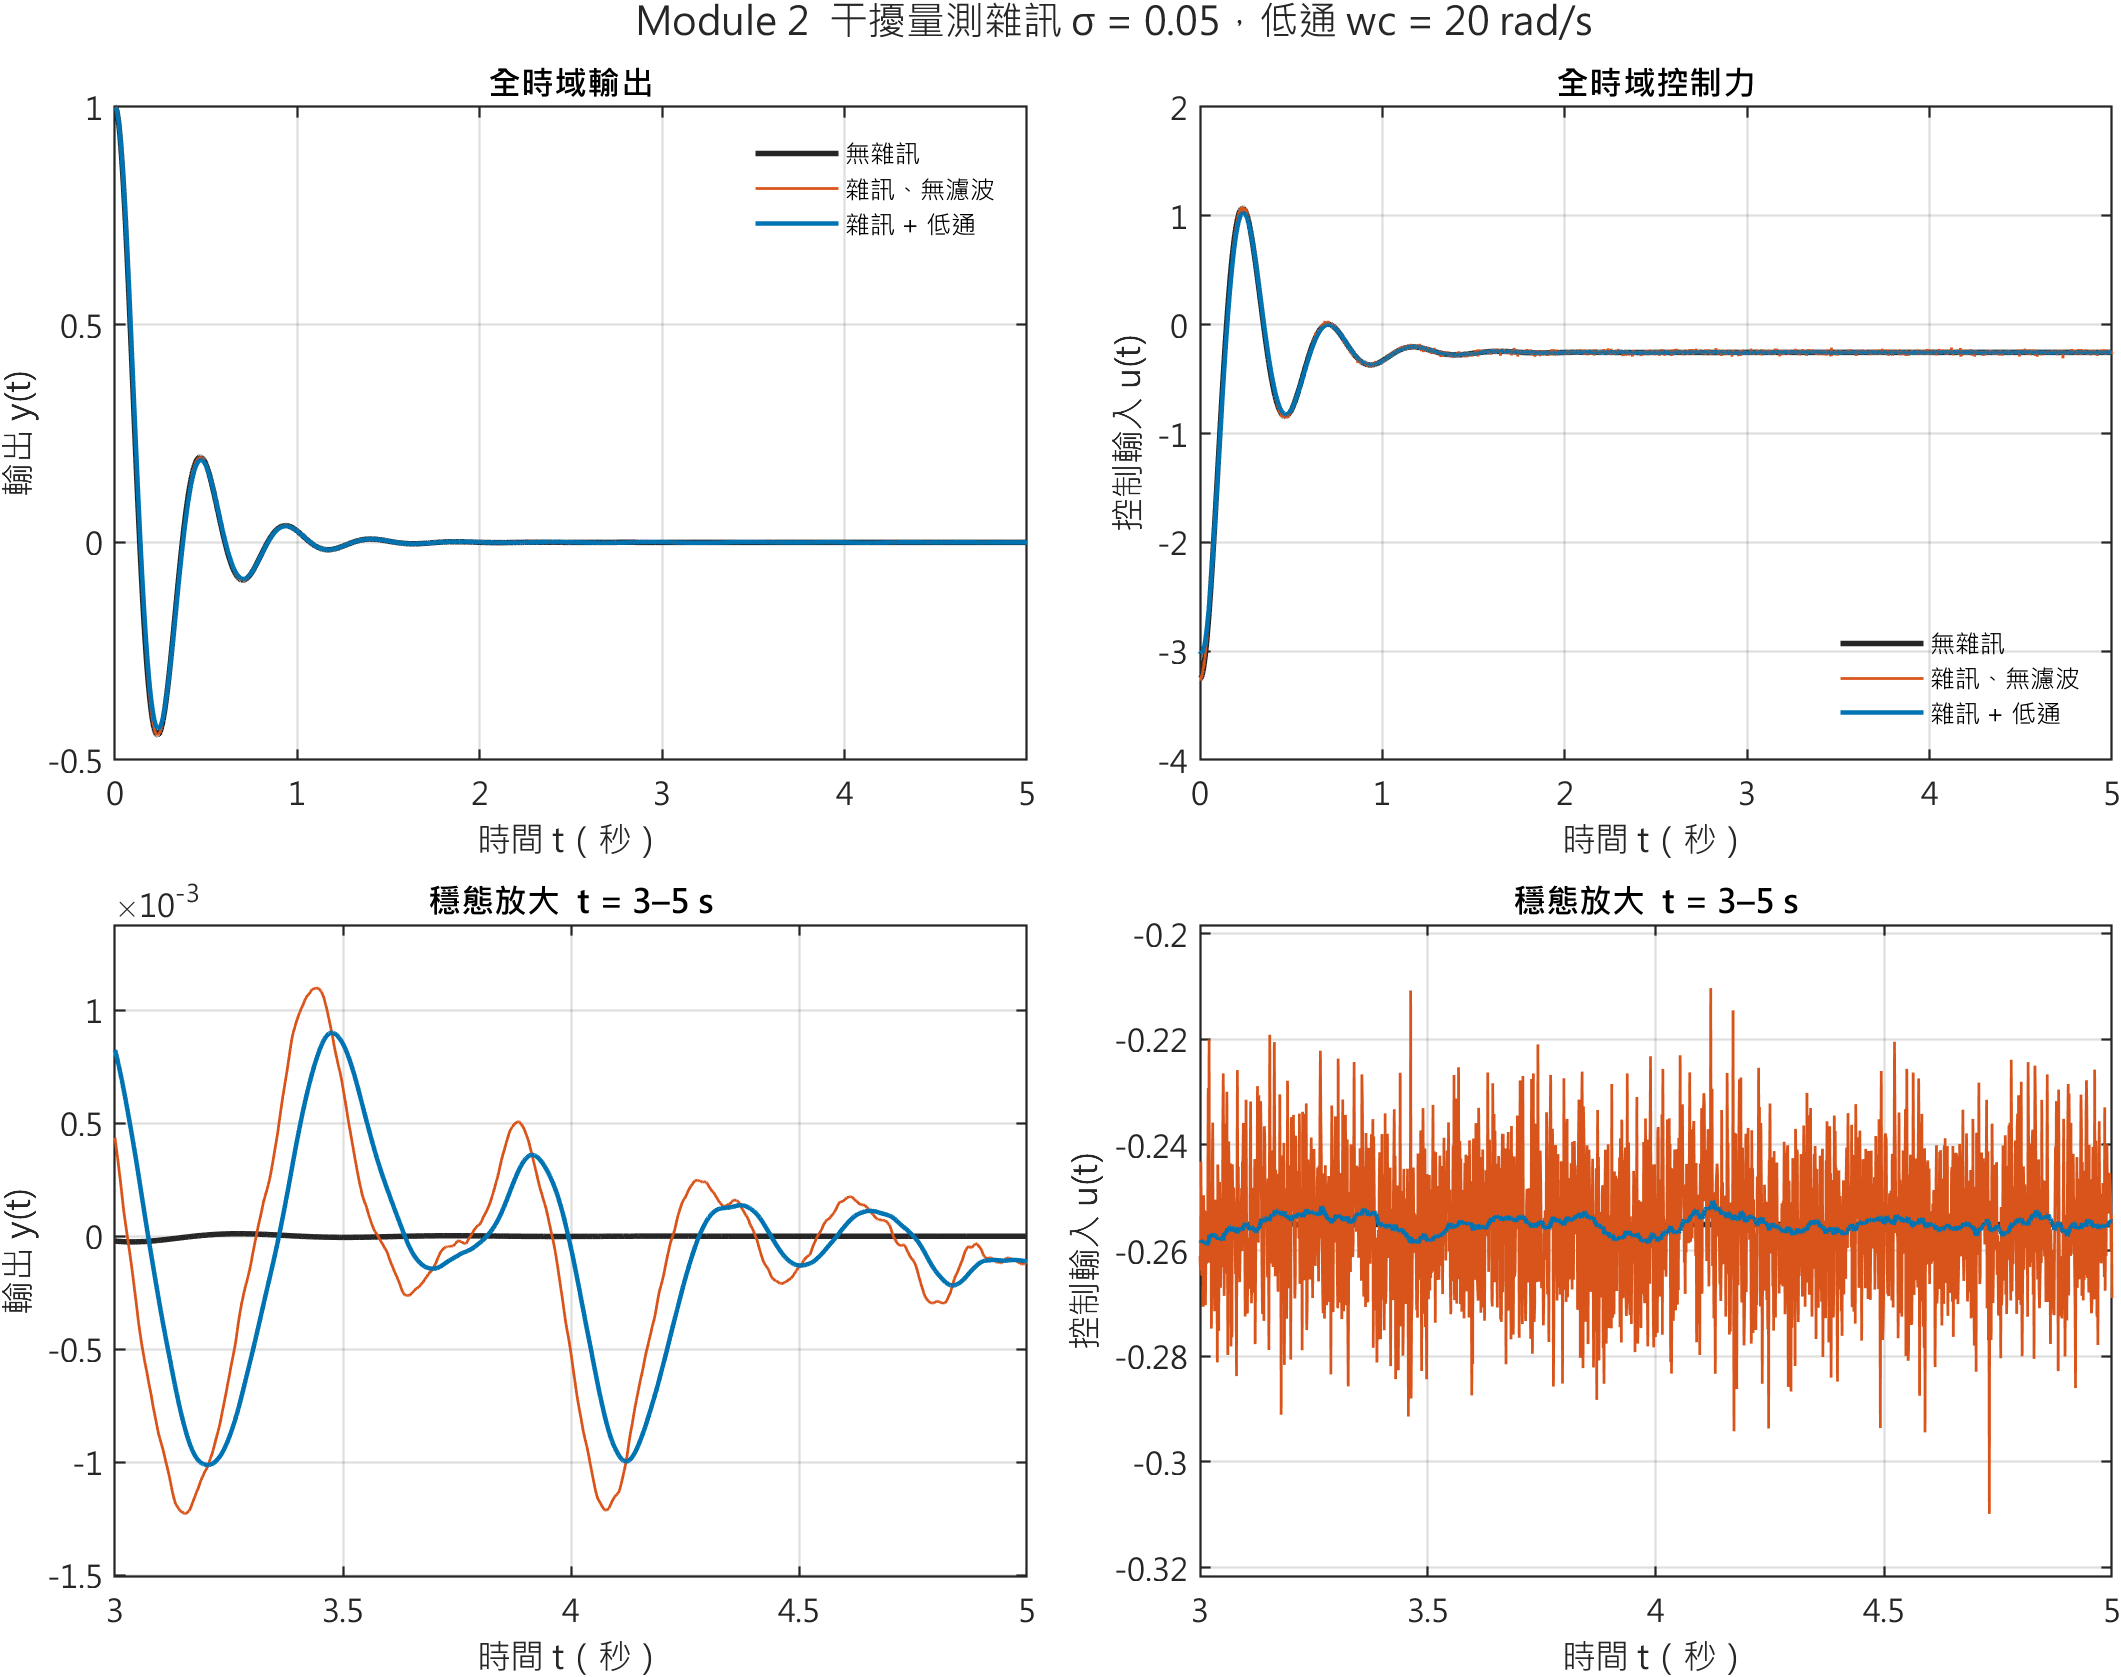
\includegraphics[width=\textwidth]{fig2_sensor_noise.png}
  \caption{Disturbance-sensor noise, \(\sigma=0.05\), and the low-pass \(20/(s+20)\).
  The upper row uses the full scale of the spike. The lower row is \([3,5]~\mathrm{s}\) only; the output scale there is \(10^{-3}\).
  Actuator chatter is obvious in \(u\). The speed barely moves.}
  \label{fig:noise}
\end{figure}

Table~\ref{tab:noise} matches that estimate: the unfiltered steady jitter of \(u\) is \(0.01292\), against \(K_{ff}\sigma=0.01275\).
The full-horizon rms values \(0.4885\) and \(0.4887\) do not reveal the noise. They are set by the swing from \(u(0^+)=-3.255\) down toward \(-K_{ff}\).
The lower-right panel of Fig.~\ref{fig:noise} is the measurement that matters.
The low-pass cuts the steady jitter of \(u\) from \(0.01292\) to \(0.00149\), a factor of \(8.7\), and it slightly lowers the speed jitter, from \(5.05\times 10^{-4}\) to \(4.41\times 10^{-4}\).
The speed was already quiet. Relative degree \(2\) filters \(n\) before it can move \(y\), which is why the lower-left panel lives on a scale of \(10^{-3}\) while \(u\) chatters by several hundredths.

The filter is not free. It also delays the genuine step in \(w\).
The initial feedforward kick is no longer a step of height \(K_{ff}\), so \(\max|u|\) falls from \(3.255\) to \(3.020\) and the undershoot shrinks from \(-0.443\) to \(-0.428\).
Those two changes are deterministic, not a reduction of random chatter.
A specification that looked only at the full-horizon rms of \(u\) would credit the filter with a noise improvement of \(0.4887\) versus \(0.4769\), which is mostly the smaller initial transient.
The actuator benefit that belongs to the noise is the steady-state column.

%==============================================================================
\section{Four architectures at a +15 percent gain error}
\label{sec:arch}

The last experiment puts a \(+15\%\) gain error on the motor and runs one input history for four controllers: pure P, P with static feedforward, pure PI, and PI with the same static feedforward.
The reference is a unit step at \(t=0\). The output disturbance is a unit step at \(t=2.5~\mathrm{s}\).
Both feedforward coefficients, when present, remain the nominal \(K_{ff}\).
Figure~\ref{fig:arch} is the comparison. The poles on this mismatched plant are
\begin{align*}
  \text{P and P+FF:}&\quad -3.4890\pm 14.4051j,
  &&\omega_n=14.822,\ \zeta=0.235,\\
  \text{PI and PI+FF:}&\quad -2.8469\pm 14.2921j,\ -1.2843,
  &&\omega_n=14.573,\ \zeta=0.195.
\end{align*}
Feedforward does not change either set. The tracking zero does change: pure PI has its zero at \(-k_i/k_p=-1.333\), and PI plus feedforward moves it to \(-k_i/(k_p+K_{ff})=-1.229\).

Before the disturbance, \(w=0\).
The theoretical steady errors are \(0.068841\) for pure P, \(-0.010326\) for P plus feedforward, and \(0\) for both PI laws.
The corresponding steady inputs are \(0.2065\), \(0.2241\), and \(1/G_{\mathrm{act}}(0)=0.2218\).
The samples at \(t=2.4~\mathrm{s}\) in Table~\ref{tab:track} have already reached those values.
After \(t=2.5~\mathrm{s}\) the situation is different. If \(r(\infty)=w(\infty)=1\), then \(y=1\) and \(u=0\) satisfies both the plant and \eqref{eq:law} for every one of the four controllers: the output disturbance itself supplies the commanded speed, the tracking error is zero, and the two feedforward terms cancel.
Table~\ref{tab:rec} is that common equilibrium seen at \(t=5~\mathrm{s}\), together with the path taken to reach it.

\begin{table}[H]
  \centering
  \caption{Tracking phase at \(+15\%\) gain error, read at \(t=2.4~\mathrm{s}\), before the disturbance. Overshoot uses the theoretical phase-1 steady speed and the peak on \([0,2.5)~\mathrm{s}\).}
  \label{tab:track}
  \small
  \setlength{\tabcolsep}{4pt}
  \begin{tabular}{lrrrrr}
    \toprule
    Architecture & \(e_{ss}\) theory & \(e(2.4)\) & \(u(2.4)\) & Overshoot & \(y_{\mathrm{peak}}\) \\
    \midrule
    Pure P            & \(+0.06884\) & \(+0.06863\) & \(0.2059\) & \(46.72\%\) & \(1.366\) \\
    P + feedforward   & \(-0.01033\) & \(-0.01056\) & \(0.2234\) & \(46.72\%\) & \(1.482\) \\
    Pure PI           & \(0\)        & \(+0.00078\) & \(0.2189\) & \(48.62\%\) & \(1.486\) \\
    PI + feedforward  & \(0\)        & \(-0.00316\) & \(0.2191\) & \(59.46\%\) & \(1.595\) \\
    \bottomrule
  \end{tabular}
\end{table}

\begin{table}[H]
  \centering
  \caption{Disturbance entry at \(t=2.5~\mathrm{s}\) and the state at \(t=5~\mathrm{s}\). The jump \(y(2.5^+)-y(2.5^-)\) is \(1\) in every row. \(T_{\mathrm{rec}}\) is the time after \(2.5~\mathrm{s}\) until \(|y-1|\) stays below \(0.02\).}
  \label{tab:rec}
  \small
  \setlength{\tabcolsep}{4pt}
  \begin{tabular}{lrrrrrr}
    \toprule
    Architecture & \(y(2.5^-)\) & \(y(2.5^+)\) & \(y_{\min}\) after \(2.5\) & \(T_{\mathrm{rec}}\) (s) & \(e(5)\) & \(\max|u|\) \\
    \midrule
    Pure P            & \(0.9312\) & \(1.9312\) & \(0.5649\) & \(1.109\) & \(+5\times 10^{-5}\)  & \(3.000\) \\
    P + feedforward   & \(1.0104\) & \(2.0104\) & \(0.5279\) & \(1.124\) & \(+6\times 10^{-5}\)  & \(3.255\) \\
    Pure PI           & \(0.9989\) & \(1.9989\) & \(0.5125\) & \(1.386\) & \(-1.0\times 10^{-3}\) & \(3.013\) \\
    PI + feedforward  & \(1.0024\) & \(2.0024\) & \(0.4065\) & \(1.202\) & \(+2.3\times 10^{-3}\) & \(3.267\) \\
    \bottomrule
  \end{tabular}
\end{table}

\begin{figure}[H]
  \centering
  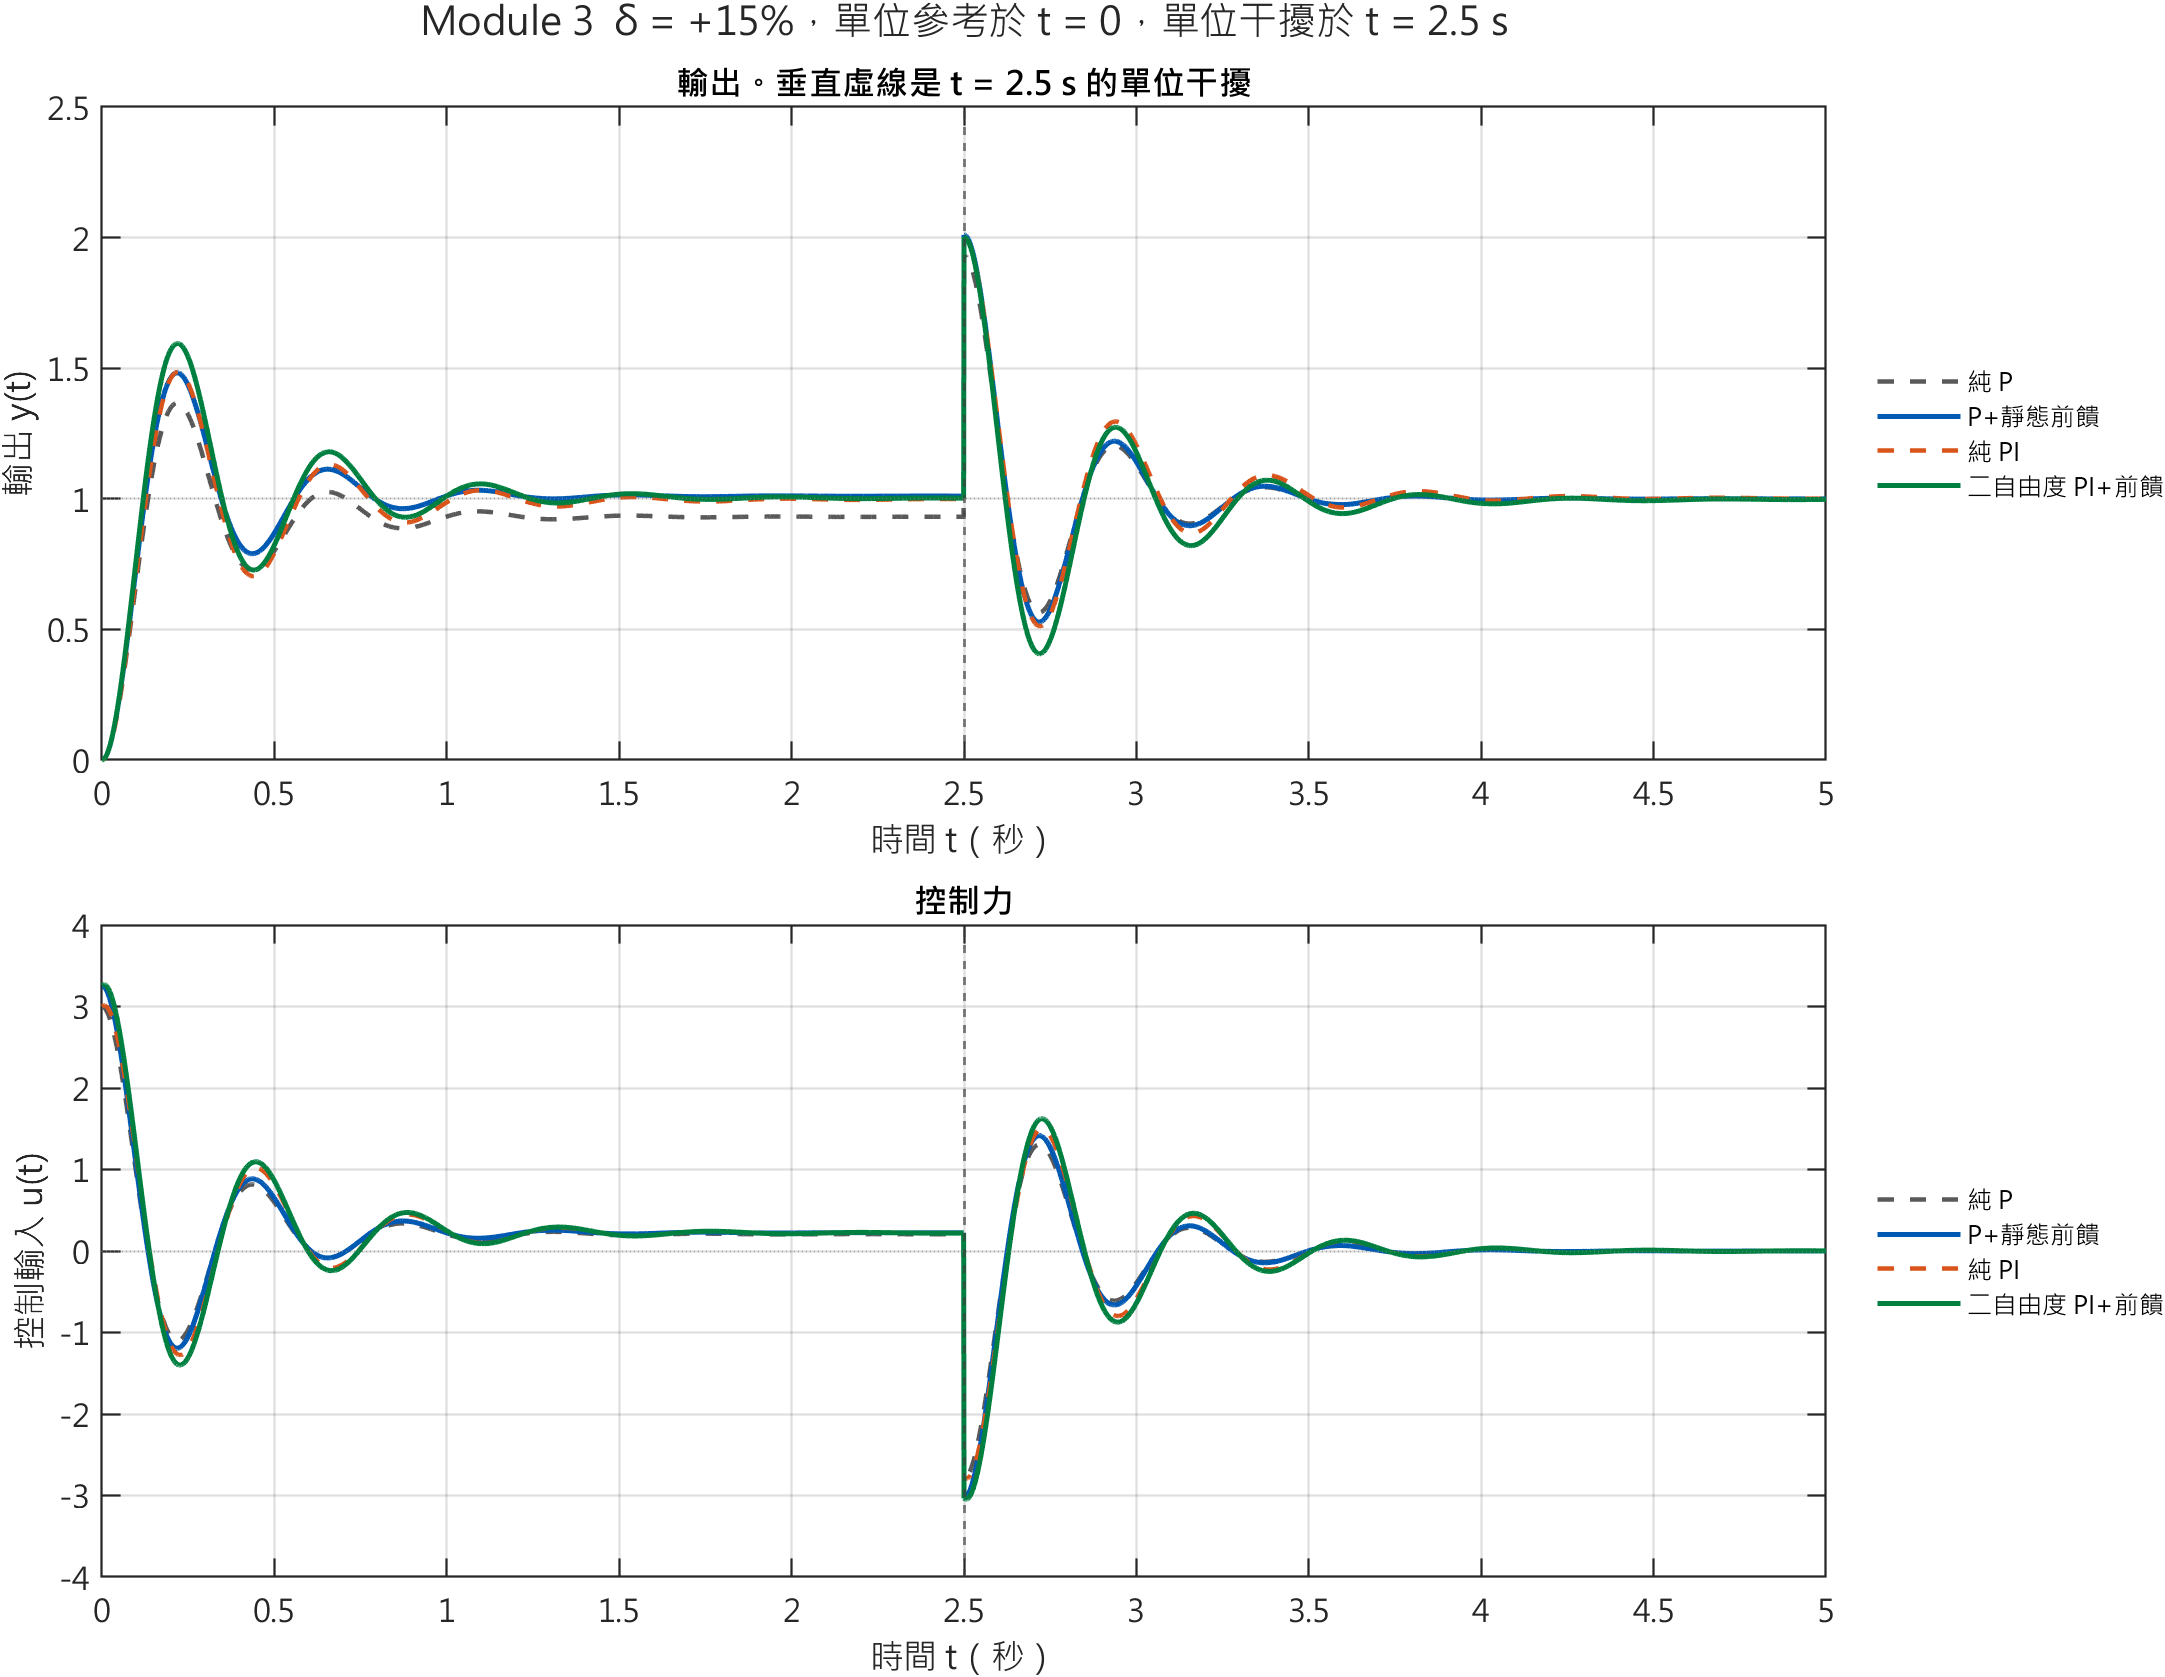
\includegraphics[width=\textwidth]{fig3_architecture_showdown.png}
  \caption{Four controllers on a motor \(15\%\) stronger than the model, with \(K_{ff}\) still equal to the nominal inverse.
  The reference steps at \(t=0\) and the output disturbance steps at the vertical line \(t=2.5~\mathrm{s}\).
  Every speed jumps by \(1\) at that line and is back near \(1\) by \(t=5~\mathrm{s}\).}
  \label{fig:arch}
\end{figure}

The tracking half of the test is where the architectures separate in steady state.
Pure P is still \(6.86\%\) low at \(t=2.4~\mathrm{s}\).
Static feedforward cuts that error to \(-1.06\%\), with the sign predicted by \eqref{eq:ess} at \(\delta=+0.15\).
The overshoot about each response's own steady value is again identical for the two proportional laws, \(46.72\%\), while the absolute peak grows from \(1.366\) to \(1.482\).
This is \eqref{eq:scale} on a hotter loop: \(\zeta\) has fallen from \(0.251\) to \(0.235\), so the percentage is a little higher than the nominal \(44.26\%\), and feedforward still does not change it.
Both PI laws are already inside a few tenths of a percent of the reference at \(t=2.4~\mathrm{s}\). The integrator, not the feedforward gain, is what removes the \(+15\%\) model error.
Adding feedforward on top of PI raises the overshoot from \(48.6\%\) to \(59.5\%\) and the peak from \(1.486\) to \(1.595\).
The poles are the same. The reference numerator changes from \(b(k_p s+k_i)\) to \(b((k_p+K_{ff})s+k_i)\). Both dc gains equal \(1\), but the larger coefficient of \(s\) drives the oscillatory pair harder, and the zero moves from \(-1.333\) to \(-1.229\).

At the disturbance the four speeds each jump by \(1.000\), from whatever value they had reached.
Pure P jumps from \(0.931\) to \(1.931\) because it was still short of the reference. The feedforward and PI speeds jump from essentially \(1\) to essentially \(2\).
The jump is the same initial-value fact as in Section~\ref{sec:spike}: the motor has no feedthrough.
Recovery is then a regulation transient back to the common equilibrium \(y=1\), \(u=0\).
By \(t=5~\mathrm{s}\) every error is a few thousandths or smaller. The proportional loops, whose slowest real part is \(-3.489\), are at about \(5\times 10^{-5}\).
The PI loops still show residuals of order \(10^{-3}\), consistent with a real pole at \(-1.284\) that has had only \(2.5~\mathrm{s}\) to decay.
Reading \(e(5)\) alone would rank the four controllers as equal. That reading is an artifact of choosing \(w_{ss}=r_{ss}\).

The recovery path is not common.
Pure P returns to the band in \(1.109~\mathrm{s}\) and bottoms at \(0.565\).
P plus feedforward takes \(1.124~\mathrm{s}\) and bottoms at \(0.528\): almost the same settling, a deeper dip, the same mechanism that deepened the nominal undershoot from \(-0.330\) to \(-0.443\).
Pure PI is the slowest return, \(1.386~\mathrm{s}\), because \(\zeta=0.195\) and the integrator state has to unwind after the jump.
PI plus feedforward shortens that return to \(1.202~\mathrm{s}\) and produces the deepest dip, \(0.407\).
The \(-K_{ff}w\) term applies the cancelling input immediately, so the integrator is left with a smaller residual to remove, while the extra kick increases the swing.
The largest \(|u|\) on \([0,5]~\mathrm{s}\) is set by the reference step, not by the disturbance: \(3.000\) for pure P, \(3.255\) for P plus feedforward, and only slightly more once an integrator is present (\(3.013\) and \(3.267\)), since \(\xi(0^+)=0\) and the integrator adds nothing to the initial sample.
Under a \(\pm 3~\mathrm{V}\) actuator limit those peaks leave the linear range. Pure P rides the rail, and both feedforward laws ask for about \(3.26\).
The deeper dip and the shorter recovery of PI plus feedforward in Table~\ref{tab:rec} both rely on that extra \(K_{ff}\) reaching the motor.
Section~\ref{sec:spike} gives the saturated initial curvature. A \(\pm 5~\mathrm{V}\) limit still contains the largest sample, \(3.267\).

Taken together, the four experiments separate three jobs that a single nominal step response ties into one number.
Static feedforward, with a correct gain, deletes the \(0.078\) steady error and \(61\%\) of the integrated absolute error, leaves the \(0.234~\mathrm{s}\) peak time and the \(44\%\) relative overshoot where they are, and increases the absolute peak from \(1.330\) to \(1.443\).
With the gain wrong by up to \(20\%\) and \(K_{ff}\) left frozen, the steady error stays inside \(2\%\) because the loop gain is \(12\), while the decay rate stays exactly \(3.489~\mathrm{s}^{-1}\) and the overshoot moves only from \(40\%\) to \(47\%\).
The unit spike at an output disturbance is structural; feedforward changes the undershoot and the settled value, and noise on that measurement reaches the actuator attenuated by \(K_{ff}\approx 0.26\). A \(20~\mathrm{rad/s}\) filter reduces the steady actuator jitter by a factor of \(8.7\) and barely moves the speed.
Under the \(+15\%\) error, integral action is what zeroes the tracking error before the disturbance arrives. Feedforward around that PI loop buys \(0.18~\mathrm{s}\) of recovery time and pays for it with a dip from \(0.51\) down to \(0.41\). The shared error at \(t=5~\mathrm{s}\) does not measure that trade.

%==============================================================================
\section{Conclusion}

With a gain error in the motor, PI plus static feedforward is the law that keeps both a zero steady tracking error and a short recovery.
The integrator clears the offset that a frozen \(K_{ff}\) leaves behind: at \(\delta=+15\%\) the speed is already within \(0.3\%\) of the reference at \(t=2.4~\mathrm{s}\).
The feedforward term then brings the output disturbance back inside the \(2\%\) band in \(1.202~\mathrm{s}\), against \(1.386~\mathrm{s}\) for PI alone.
The same term deepens the undershoot. After the disturbance the speed falls to \(0.407\), compared with \(0.512\) for PI alone and \(0.565\) for pure P.
That trade is a linear-model result. If the drive saturates near \(\pm 3~\mathrm{V}\), the initial command \(u(0^+)\approx -3.255\) clips, and both the faster recovery and the deeper undershoot have to be recomputed with the saturation included. A \(\pm 5~\mathrm{V}\) rail still contains every peak in this study.

The disturbance sensor needs a low-pass filter of its own.
A measurement noise of standard deviation \(0.05\) reaches the armature attenuated by \(K_{ff}\), and the steady jitter of \(u\) is still \(0.0129\), while the speed jitter stays near \(5\times 10^{-4}\).
The filter \(20/(s+20)\) cuts the actuator jitter by a factor of \(8.7\).
On a physical motor that filtering belongs in the design: the high-frequency component chatters and heats the drive while leaving the regulated speed almost unchanged.
\end{document}
